\chapter{Considerações Finais}\label{cap:cons_finais}

% Moved to conclusão
\section{Trabalhos Futuros}

O trabalho atual pode permitir que um time melhor seja criado modificando-se os
parâmetros da função objetivo ou adicionando novos custos à função objetivo.
Assim, o modelo de competição apresentado na Figura~\ref{fig:mod_comp} pode ser
utilizado.

\begin{figure}[H]
  \centering
  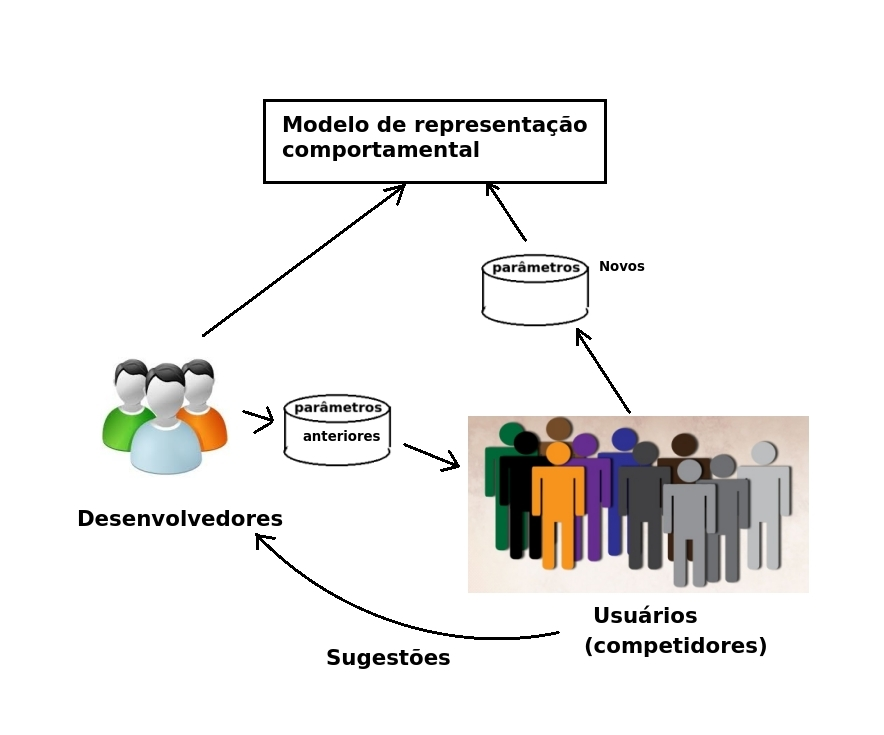
\includegraphics[width=0.8\linewidth]{mod_comp}
  \caption{Modelo de Competição para melhorar
           o time}\label{fig:mod_comp}
\end{figure}

Dessa forma, através do fornecimento dos parâmetros vencedores da competição
anterior, tem-se um avanço no desempenho do time.

Outra forma de se melhorar o time é utilizar uma maneria automática para
realizar as partidas e avaliar o desempenho do time nessa partida. Isso
permitiria que algorítimos de otimização também fossem utilizados para melhorar
os parâmetros.  Uma das dificuldades desta abordagem é a necessidade de se
alterar o simulador para reposicionar a bola ou os robôs durante a partida.

% OBS: As expected, there are x'es everywhere here after revision...
%      So we are removing this section...
%\section{Dificuldades}
%
%A principal dificuldade foi criar os parâmetros da função objetivo e
%ajusta-los para se ter um bom desempenho. Isso, pois o espaço de busca dos
%parâmetros aumenta a cada parâmetro adicionado, complicando o ajuste dos
%parâmetros.
%
%Conforme citado na Seção~\ref{sec:defs}, o nível de complexidade das ações
%modeladas influi diretamente no número de ações que poderão ser consideradas a
%tempo de serem úteis para o jogo real.
%
%Como a complexidade cresce exponencialmente, onde o número de ações básicas é a
%base, conforme~\cite{russell2003artificial}, temos a Equação~\ref{eq:cres_exp}.
%
%\begin{dmath}\label{eq:cres_exp}
% número{\ }de{\ }estados = num \lbrace A^i \rbrace ^{profundidade}
%\end{dmath}
%
%Isso não é um problema que pode ser tratado simplesmente com o aumento da
%velocidade de processamento. Deve-se ajustar o nível de abstração de acordo com
%os resultados obtidos nos teste práticos.
%
%Quanto mais ações, maior é o custo computacional. Por isso, talvez seja mais
%relevante investir em soluções envolvendo teoria dos jogos. Com vários níveis de
%jogadas mais simples, jogadas mais complexas como passes surgem de chutes e
%movimentações. Isso simplificaria a função objetivo, reduzindo o custo da
%avaliação. Também, apesar de se ter um crescimento exponecial, pode-se aplicar
%métodos de poda da busca para reduzir os nós considerados (vide
%\cite{russell2003artificial}).
%
%Outro fator importante é a maneira como os estados são expandidos. Isso afeta a
%convergência e, como consequência, o desempenho em tempo real. Pode-se mover
%mais de um robô em cada ramo da busca, mas talvez seja mais relevante mover
%somente um robô por aresta. Isso, contudo, deve ser considerado no modelo para
%manter a coerência do planejamento.  Ficou evidente a importância da modelagem
%do jogo no desempenho do planejamento.
%
%Por fim, um problema fundamental para um bom desempenho é o controle.  Fator que foi
%evidenciado nos testes com o simulador, afetando o desempenho do time. A importância
%deste problema fica clara quando um planejamento que custou tempo e recursos computacionais
%não é executado corretamente. Um planejamento não tem utilidade quando não é válido
%no mundo real. Por exemplo, se um passe resultar em um gol no planejamento, mas não
%for executado corretamente, perde-se a posse de bola.

% vim: tw=80 et ts=2 sw=2 sts=2 ft=tex
